%----------------------------------------------------------------------------------------
%	PACKAGES AND OTHER DOCUMENT CONFIGURATIONS
%----------------------------------------------------------------------------------------

\documentclass[landscape,archE1,fontscale=0.285]{baposter} % Adjust the font scale/size here

\usepackage{graphicx} % Required for including images
\graphicspath{{figures/}} % Directory in which figures are stored

\usepackage{amsmath} % For typesetting math
\usepackage{amssymb} % Adds new symbols to be used in math mode

\usepackage{float}
\usepackage{booktabs} % Top and bottom rules for tables
\usepackage{enumitem} % Used to reduce itemize/enumerate spacing
\usepackage{palatino} % Use the Palatino font
\usepackage[font=small,labelfont=bf]{caption} % Required for specifying captions to tables and figures

\usepackage{multicol} % Required for multiple columns
\setlength{\columnsep}{1.5em} % Slightly increase the space between columns
\setlength{\columnseprule}{0mm} % No horizontal rule between columns

\usepackage{tikz} % Required for flow chart
\usetikzlibrary{shapes,arrows} % Tikz libraries required for the flow chart in the template

\newcommand{\compresslist}{% Reduce spacing within itemize/enumerate environments
\setlength{\itemsep}{1pt}
\setlength{\parskip}{0pt}
\setlength{\parsep}{0pt}
}

\definecolor{lightblue}{rgb}{0.145,0.6666,1} % Defines the color used for content box headers

\begin{document}

\begin{poster}
{
headerborder=closed, % Adds a border around the header of content boxes
colspacing=1em, % Column spacing
bgColorOne=white, % Background color for the gradient on the left side of the poster
bgColorTwo=white, % Background color for the gradient on the right side of the poster
borderColor=lightblue, % Border color
headerColorOne=black, % Background color for the header in the content boxes (left side)
headerColorTwo=lightblue, % Background color for the header in the content boxes (right side)
headerFontColor=white, % Text color for the header text in the content boxes
boxColorOne=white, % Background color of the content boxes
textborder=roundedleft, % Format of the border around content boxes, can be: none, bars, coils, triangles, rectangle, rounded, roundedsmall, roundedright or faded
eyecatcher=true, % Set to false for ignoring the left logo in the title and move the title left
headerheight=0.155\textheight, % Height of the header
headershape=roundedright, % Specify the rounded corner in the content box headers, can be: rectangle, small-rounded, roundedright, roundedleft or rounded
headerfont=\Large\bf\textsc, % Large, bold and sans serif font in the headers of content boxes
%textfont={\setlength{\parindent}{1.5em}}, % Uncomment for paragraph indentation
linewidth=2pt % Width of the border lines around content boxes
}
%----------------------------------------------------------------------------------------
%	TITLE SECTION 
%----------------------------------------------------------------------------------------
{
\includegraphics[height=12em]{figures/Inst-Prim-FulClr.png}} % First university/lab logo on the left
{\bf\textsc{Computational Evalutions of Proton Induced Gain in a Portable Faraday Cup}} % Poster title
{\textsc{Shaun Marshall$^{1\dag}$, Blake Currier$^1$, Andrew Hodgdon$^2$ \\$^1$Department of Physics, Worcester Polytechnic Institute, Worcester, MA 01609\\ $^2$RadSim, LLC, Newton, MA 02462}} \\ % Author names and institution
%{
\includegraphics[height=4em]{logo.png}} % Second university/lab logo on the right

%----------------------------------------------------------------------------------------
%	ABSTRACT
%----------------------------------------------------------------------------------------

\headerbox{{\fontsize{18}{18}\selectfont Abstract}}{name=abstract,column=0,row=0,above=bottom}{

\begin{itemize}[leftmargin=*]\compresslist
\item {\fontsize{15}{18}\selectfont Current proton beam\\calibration methods lack\\precision, esp. for pencil-beam scanning}
\item {\fontsize{15}{18}\selectfont Seek feasible (vacuumless, chamberless) solution for $70 - 250 MeV$ beam energy:\\\fontsize{14.5}{17}\selectfont Portable Faraday Cup (PFC)}
\end{itemize}

\begin{center}
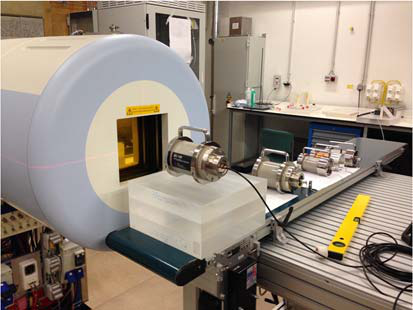
\includegraphics[width=0.7\linewidth]{figures/HIT_setup.png}
%\captionof{figure}{{\fontsize{15}{18}\selectfont Experimental beamline at Heidelberg Institute of Technology}}
\\{\fontsize{12.5}{16}\selectfont \textbf{Fig 1:} Experimental beamline at Heidelberg Institute of Technology}
\end{center}

\begin{itemize}[leftmargin=*]\compresslist
\item {\fontsize{15}{18}\selectfont Kapton insulator to capture backscattered electrons}
\item {\fontsize{15}{18}\selectfont PFC radius determined by MCNP6 model}
\end{itemize}

\begin{center}
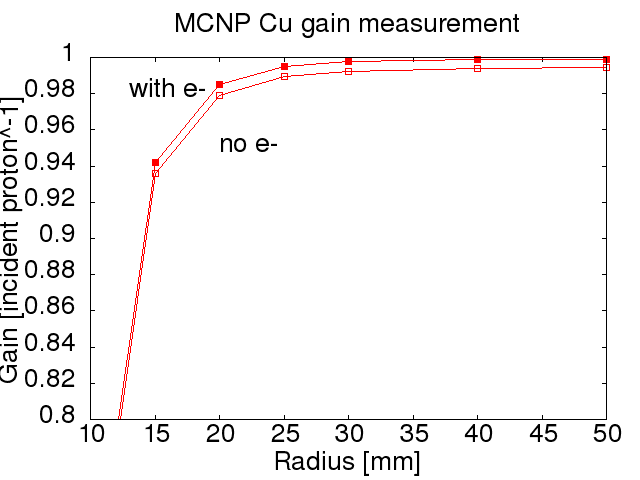
\includegraphics[width=0.75\linewidth]{figures/MCNP_gain_radius.png}
%\captionof{figure}{MCNP device radius gain optimization}
\\{\fontsize{14.5}{16}\selectfont \textbf{Fig 2:} MCNP gain as a function of PFC radius}
\end{center}
}

%----------------------------------------------------------------------------------------
%	METHODOLOGY
%----------------------------------------------------------------------------------------

\headerbox{{\fontsize{18}{18}\selectfont Methodology}}{name=methodology,column=1,row=0,above=bottom,aligned=abstract}{

{\fontsize{15}{18}\selectfont \textbf{PFC Geometry}}
\begin{itemize}[leftmargin=*]\compresslist
\item {\fontsize{15}{18}\selectfont Cu cylinder (10cm x 3 cm)}
\item {\fontsize{15}{18}\selectfont Kapton film (59-200 $\mu$m)}
\item {\fontsize{15}{18}\selectfont Ag ground (12 $\mu$m)}
\item {\fontsize{15}{18}\selectfont Kapton outer film (62 $\mu$m)}
\end{itemize}
\begin{center}
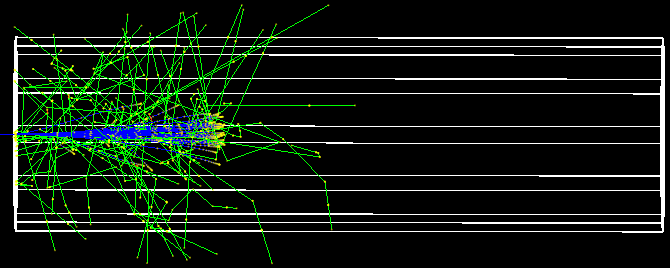
\includegraphics[width=0.9\linewidth]{figures/G4_dist.png}
%\captionof{figure}{Geant4- 100 events at 160 MeV in S59}
\\{\fontsize{14.5}{16}\selectfont \textbf{Fig 3:} Geant4- 100 events at 160 MeV in S59}
\end{center}
\vspace{1em}
{\fontsize{15}{18}\selectfont \textbf{Gain Contribution}}
\begin{itemize}[leftmargin=*]\compresslist
\item {\fontsize{15}{18}\selectfont Net charge on Cu per p+}
\item {\fontsize{15}{18}\selectfont Mirror charge $\propto$ depth in Kapton $d_{\%,j}$}
\item {\fontsize{15}{18}\selectfont For each charge $q_j$ per event $i$, tally net gain}
  $$ g_{ij} = \left\{\begin{array}{ll}
                  \pm q_j/e, & \text{if } q_j \rightleftharpoons Cu \\
                  \pm q_jd_{\%,j}/e, & \text{if } q_j \rightleftharpoons KA(d_{\%,j})
                  \end{array}\right.$$
\end{itemize}
\vspace{1em}
{\fontsize{15}{18}\selectfont \textbf{Parameters}}
\begin{itemize}[leftmargin=*]\compresslist
\item {\fontsize{15}{18}\selectfont Energy range: $70 - 250 MeV$}
\item {\fontsize{15}{19}\selectfont Beam FWHM: $22.8 - 8.1 mm$}
\item {\fontsize{15}{18}\selectfont Production cutoff: 5 $\mu$m}
\item {\fontsize{15}{18}\selectfont Models: S59, S100, S200\\(Kapton thicknesses)}
\end{itemize}
}

%----------------------------------------------------------------------------------------
%       RESULTS
%----------------------------------------------------------------------------------------

\headerbox{{\fontsize{18}{18}\selectfont Results}}{name=results,column=2,row=0,above=bottom,aligned=abstract}{

\begin{center}
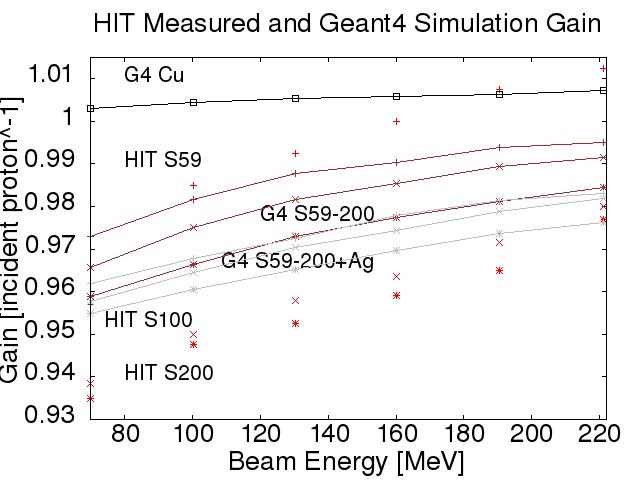
\includegraphics[width=0.8\linewidth]{figures/G4_HIT_gain.png}
%\captionof{figure}{G4, HIT gain measurements \cite{Gordan:2014}, all increase with beam energy.  Cu exhibits positive gain, KA lowers gain with thickness; Ag lowers gain, suppresses this spread. HIT-S59 breaks trend, crosses 1.}
\\{\fontsize{13.5}{14}\selectfont \textbf{Fig 4:} G4, HIT gain \cite{Gordan:2014}, all increase with energy.  Cu shows positive gain, KA lowers gain with thickness; Ag lowers gain, suppresses this spread. HIT-S59 breaks trend, crosses 1.}
\end{center}
\vspace{-1em}
\begin{table}[H]
\centering
\begin{tabular}{cccc}
\toprule
& S59 & S100 & S200 \\
\midrule
-Ag & $1.1-3.0$ & $1.4-3.7$ & $2.0-4.4$ \\
+Ag & $2.4-4.1$ & $2.5-4.5$ & $2.9-4.8$ \\
\bottomrule
\end{tabular}
\\{\fontsize{14}{14}\selectfont \textbf{Table 1:} G4 model gain percent error relative to G4 Cu}
\end{table}

\begin{center}
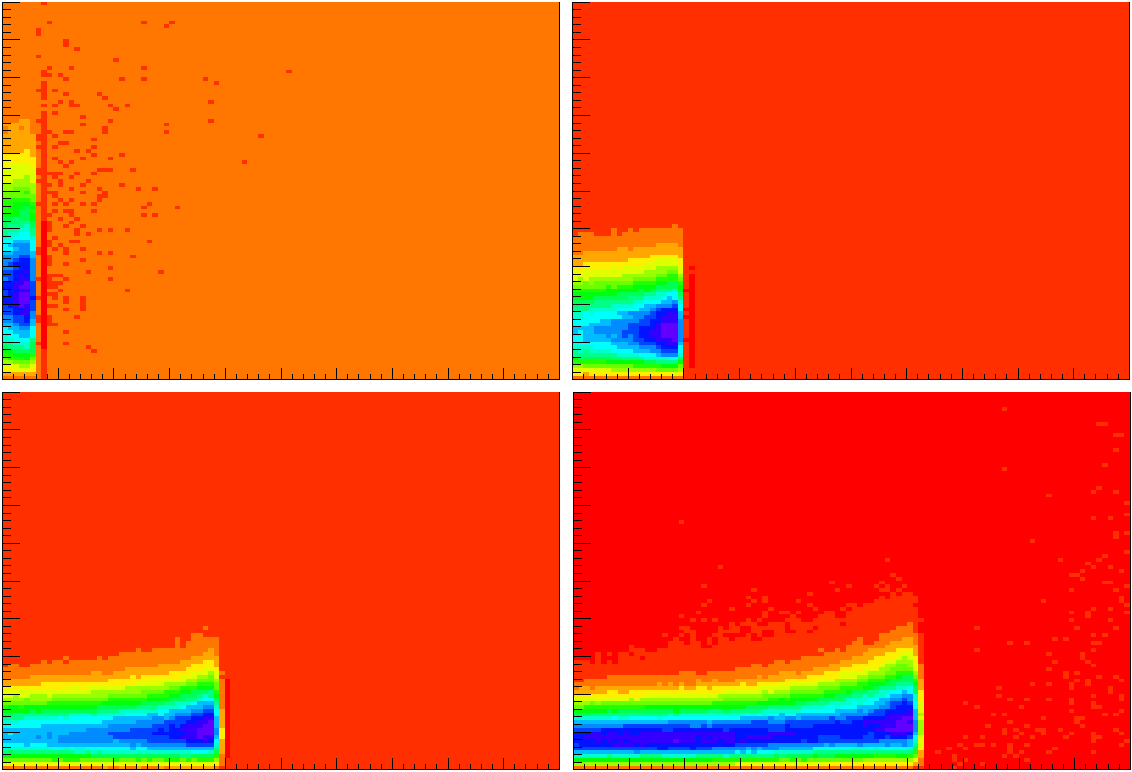
\includegraphics[width=0.77\linewidth]{figures/G4_Cu_gain.png}
%\captionof{figure}{G4 gain 100x100 bin histogram at a) 70 MeV, b) 130 MeV, c) 190 MeV, d) 250 MeV.  Each bin adds charge values at end locations and subtracts at production.  Colormap varies from red (positive) to blue (negative) (unnormalized).}
\\{\fontsize{13.5}{14}\selectfont \textbf{Fig 5:} G4 gain in 100x100 bins at 70, 130, 190, 250 MeV.  Bins append charge deposits (red) and subtract removals (blue) (unnormalized).}
\end{center}

}

%----------------------------------------------------------------------------------------
%	CONCLUSIONS
%----------------------------------------------------------------------------------------

\headerbox{{\fontsize{18}{18}\selectfont Conclusions}}{name=conclusions,column=3,row=0,aligned=abstract}{

\begin{center}
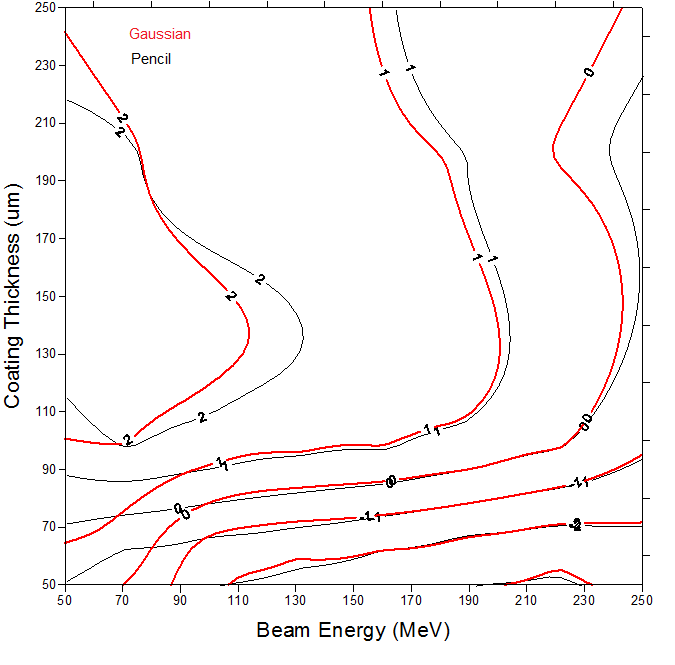
\includegraphics[width=0.7\linewidth]{figures/G4_HIT_errorPencilGauss.png}
%\captionof{figure}{G4, HIT gain \% error contours}
\\{\fontsize{13}{16}\selectfont \textbf{Fig 5:} G4, HIT gain \% error}
\end{center}
\vspace{-2em}
\begin{itemize}[leftmargin=*]\compresslist
\item {\fontsize{15}{18}\selectfont Agreement within 3\%}
\item {\fontsize{15}{18}\selectfont MCNP insufficient to\\optimize without p+\\secondary electrons}
\item {\fontsize{15}{18}\selectfont Future work: characterize multilayer PFC}
\end{itemize}
}

%----------------------------------------------------------------------------------------
%	CONTACT INFORMATION
%----------------------------------------------------------------------------------------

\headerbox{{\fontsize{18}{18}\selectfont $^\dag$Contact Info}}{name=contact,column=3,above=bottom}{

\begin{description}\compresslist
\item[Web] www.wpi.edu/$\sim$shaun
\item[Email] shaun@wpi.edu
\end{description}
}

%----------------------------------------------------------------------------------------
%	REFERENCES
%----------------------------------------------------------------------------------------

\headerbox{{\fontsize{18}{18}\selectfont References}}{name=references,column=3,above=contact,below=conclusions}{

\renewcommand{\section}[2]{\vskip 0.0em} % Get rid of the default "References" section title
\nocite{*} % Insert publications even if they are not cited in the poster
\small{ % Reduce the font size in this block
\bibliographystyle{unsrt}
\bibliography{refs} % Use refs.bib as the bibliography file
}}

\end{poster}

\end{document}

%%%%%%%%%%%%%%%%%%%%%%%%%%%%%%%%%%%%%%%%%%%%%%%%%%%%%%%%%%%%%%%%%%%%%
% baposter Class Created by:
% Brian Amberg (baposter@brian-amberg.de)
%
% License:
% CC BY-NC-SA 3.0 (http://creativecommons.org/licenses/by-nc-sa/3.0/)
%%%%%%%%%%%%%%%%%%%%%%%%%%%%%%%%%%%%%%%%%%%%%%%%%%%%%%%%%%%%%%%%%%%%%
